\section{Эволюция подходов к решению задачи SOD}

\begin{figure}
    \centering
    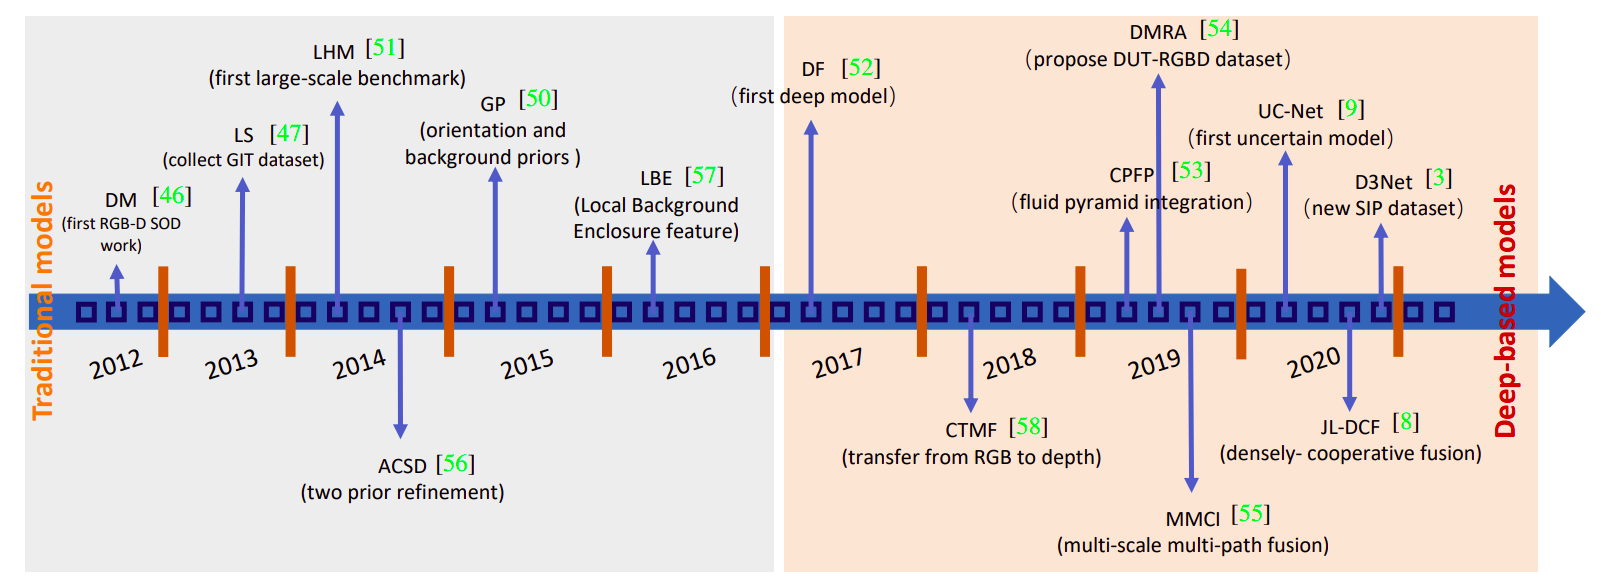
\includegraphics[width=1\textwidth]{chronology}
    \caption{Хронология развития подходов к решению задачи RGB-D SOD}
    \label{fig:chronology}
\end{figure}

Задача SOD привлекает внимание исследователей уже долго время. Применение карты глубины для выявления заметных объектов на изображении 
внесло ещё больше разнообразие в обширный список подходов для решения этой задачи. Разделяют традиционные методы и методы, основанные 
на использовании глубоких нейронных сетей. На схеме \ref{fig:chronology} из работы \cite{Survey} можно увидеть краткую хронологию развития
подходов к решению задачи RGB-D SOD.


Традиционные алгоритмы, не использующие нейронные сети, основаны на извлечении и анализе заранее определенных признаков RGB изображения и соответствующей ему карты глубины.
Например, такими признаками может быть контрастность, цвет или границы определённой части изображения. 
В работе \cite{Depth-really-Matters} была предложена модель, использующая геометрические признаки поверхностей объектов в помещении и глубину. 
А в работе \cite{Depth-View-of-Saliency} для расчета заметности объекта используют цветовой контраст и вычисление нормали к поверхности\cite{Surface-Normal} для каждого пикселя на изображении.

\begin{figure}
    \centering
    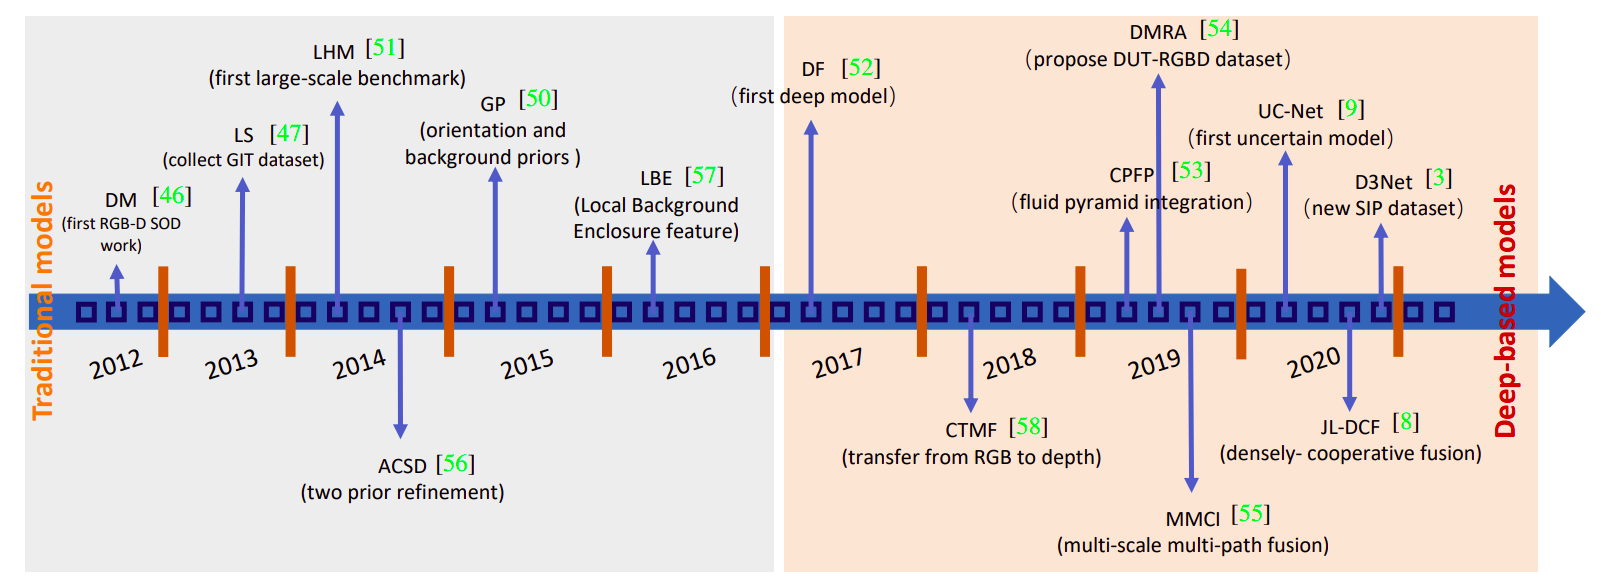
\includegraphics[width=1\textwidth]{chronology}
    \caption{Процесс обработки изображения, предложенный в работе \cite{RGBD-SOD-Deep-Fusion}}
    \label{fig:pipeline}
\end{figure}

С развитием глубоких нейронных сетей на смену традиционным подходам к решению задачи SOD пришли модели, основанные на различных архитектурах нейронных сетей.
Так, в работе \cite{RGBD-SOD-Deep-Fusion} была предложена модель DF на основе свёрточной нейронной сети (CNN). Однако модель применялась не к сырому изображению, 
а к предварительно подготовленным признакам. Из извлечённых признаков формировались каналы изображения, которые и передавались в нейронную сеть, которая, в свою очередь,
выявляла самый заметный регион на картинке. Процесс обработки изображения и применение модели изображены на схеме \ref{fig:pipeline}


Последующие предложенные модели использовали более современный end-to-end подход к использованию CNN, предоставляя нейронной сети самой извлекать 
и высокоуровневые, и низкоуровневые признаки с изображений самостоятельно, без предварительных ручных шагов.
В отличие от заранее заданных признаков, признаки, извлекаемые нейронной сетью, содержат больше семантической информации об объектах на изображении, а значит
позволяют точнее решать задачи, для которых необходимое "понимать" изображённую сцену. 

Первой моделью, использующей только свёрточные сети для извлечения признаков, стала модель CTMF \cite{CNNs-Based}. 
Следующие работы представляли эксперименты с различными архитектурами сетей и различными подходами 
к совместной обработке извлечённых признаков из RGB изображении и карты глубины. В \cite{Progressively} для обработки 
изображения и карты глубины авторы применяют две различные сети, а затем сливают 2 карты признаков в одну и 
на её основе модель делает предсказание. А в работе \cite{Single-Stream} авторы предлагают противоположный предыдущему 
single-stream подход к обработке изображения и его карты глубины с помощью архитектуры Single Stream Recurrent Convolution Neural Network(SSRCNN),
принимающей на вход 4 канала: 3 канала отвечают за RGB изображение, 4-й - за карту глубины.

Некоторые работы предлагают способы борьбы с зашумлённой картой глубины, которая может существенно повлиять на качество модели.
Например, в \cite{Contrast} был предложен метод по увеличению контрастности карты глубины. А в \cite{Rethinking-RGBD} был предложен 
способ автоматической оценки качества карты глубины и отфильтровывания карт плохого качества.

Кроме моделей, архитектуры которых основаны на свёрточных нейронных сетях, для задачи RGB-D SOD предлагаются и другие решения. 
Например, модель UC-Net, предложенная в работе \cite{UC-Net}, представляет собой вероятностную модель, основанную надо
вариационный автокодировщик(VAE), чтобы эмулировать неопределённость выбора человека во время выделения самого заметного объекта.
Для каждого входа модель генерирует сразу несколько карт значимости (saliency maps) путём сэмплирования из скрытого пространства,
сформированного при обучении модели.


В данной работе мы сосредоточимся на модели BBS-Net\cite{BBS}, предложенной летом 2020 года и являющейся одним из State-of-the-Art подходов.
Модель использует предобученные свёрточные сети для извлечения признаков и использует специальные модули для объединения карт признаков,
полученных из RGB изображения и карты глубины. 

В следующей части мы подробнее рассмотрим устройство свёрточных нейронных сетей, а после этого детально проанализируем архитектуру BBS-Net\cite{BBS}.